\documentclass[11pt]{beamer}
\usepackage{
	xcolor,
	graphicx,
	subcaption,
	bm,
	pifont,
	booktabs,
	multirow,
	float,
	amsmath, 
	amssymb,
	appendixnumberbeamer
	} 
%\usefonttheme[onlymath]{serif} % mathmode font like in article TeX	

% https://tex.stackexchange.com/questions/565069/beamer-bold-math-no-longer-working
% allows for boldface in beamer
\DeclareFontShape{OT1}{cmss}{b}{n}{<->ssub * cmss/bx/n}{} 

	
\usetheme{Madrid}

\definecolor{emc-darkblue}{RGB}{14, 36, 112}
\definecolor{emc-lightblue}{RGB}{153, 209, 232}
\definecolor{ggray}{RGB}{208, 208, 208}


\setbeamercolor{palette primary}{bg=emc-darkblue, fg=white}
\setbeamercolor{palette secondary}{bg=emc-lightblue, fg=emc-darkblue}
\setbeamercolor{palette tertiary}{bg=emc-darkblue, fg=white}
\setbeamercolor{structure}{fg=emc-darkblue} 
\setbeamercolor{section in toc}{fg=emc-darkblue} 

\title[CITRUS]{Convergence for Individualizing TReatment Using Statistical approaches (CITRUS)}


\author[Welz, ten Haaf, Alfons]{\underline{Max Welz}\inst{1,2} \and Kevin ten Haaf\inst{2} \and Andreas Alfons\inst{1}}
\institute[]{\inst{1} Erasmus University Rotterdam, Dept. of Econometrics \and \inst{2} Erasmus Medical Center, Dept. of Public Health}

\titlegraphic{
\includegraphics[width=5cm]{eur-logo.png}}

\date[October 21, 2021]{October 21, 2021 \\\bigskip Tinbergen Institute PhD Seminar}

\pgfdeclareimage[height=0.5cm]{university-logo}{eur-stamp.png}
\logo{\pgfuseimage{university-logo}}


% Delete this, if you do not want the table of contents to pop up at
% the beginning of each section:



%%%%%%%%% bugfix for TeXShop:
\makeatletter
\let\@@magyar@captionfix\relax
\makeatother



%%%%%%%% Bibliography
% capitalization of Dutch names (function applicable to bib file)
\DeclareRobustCommand{\VAN}[3]{#3}

 
%%  bib settings
\usepackage{natbib}
\setcitestyle{authoryear} 
\bibliographystyle{apalike} 
% make bibliography entries smaller
\renewcommand\bibfont{\scriptsize}
% If you have more than one page of references, you want to tell beamer
% to put the continuation section label from the second slide onwards
\setbeamertemplate{frametitle continuation}[from second]
% Now get rid of all the colours
\setbeamercolor*{bibliography entry title}{fg=black}
\setbeamercolor*{bibliography entry author}{fg=black}
\setbeamercolor*{bibliography entry location}{fg=black}
\setbeamercolor*{bibliography entry note}{fg=black}
% and kill the abominable icon
\setbeamertemplate{bibliography item}{}



% link coloring
\usepackage{hyperref}
\hypersetup{
	hidelinks,
    colorlinks = true,
    linkbordercolor = {white},
    citecolor = emc-darkblue,
    urlcolor = black,
    linkcolor = black,
    linktoc = all % make both sections and subsections in ToC clickable
}

%%%%%%%%% For the questionnaire tables
\usepackage{array}
\usepackage{tabularx}
\newcolumntype{S}{>{\centering\arraybackslash}m{4em}}
\renewcommand{\tabularxcolumn}[1]{m{#1}} % redefine 'X' to use 'm'


%%%%%%%%% tikZ
\usepackage{tikz, latexsym}
    \usetikzlibrary{decorations.pathreplacing}
    \usetikzlibrary{fadings}
    

% Delete this, if you do not want the table of contents to pop up at
% the beginning of each section:
\AtBeginSection[]
{
    \begin{frame}
        \frametitle{Outline}
        \tableofcontents[currentsection]
    \end{frame}
}

\AtBeginSubsection[]
{
    \begin{frame}
        \frametitle{Outline}
        \tableofcontents[currentsection,currentsubsection]
    \end{frame}
}

%%%% definitions
\newcommand{\X}{\mathbf{X}}
\newcommand{\x}{\mathbf{x}}
\renewcommand{\P}{\mathbb{P}}
\newcommand{\G}{\mathcal{G}}

 
%%%% Let's get started %%%%%
\begin{document}

\begin{frame}
  \titlepage
\end{frame}

\section{Introduction}

\begin{frame}{Background}

\begin{center}
	{	\Large
	\textcolor{darkgray}{
	\textit{CITRUS  = \\ \alert{C}onvergence for \alert{I}ndividualizing \alert{TR}eatment \alert{U}sing \alert{S}tatistical approaches}}}
\end{center}

\bigskip

\begin{itemize}
	\item Project of the  Econometric Institute and Erasmus Medical Center;
	\item Part of the \href{https://convergencealliance.nl/}{\textit{\textcolor{emc-darkblue}{Convergence Alliance}}} between EUR, EMC, TU Delft; 
	\item Fully funded by an \href{https://convergencealliance.nl/granted-open-mind-calls/}{\textit{\textcolor{emc-darkblue}{Open Mind Call}}} grant (awarded: 08--12/2021).  
\end{itemize}
\end{frame}



\begin{frame}{Introduction}
\alert{Evidence-based medicine}: the \textit{``conscientious, explicit and judicious
use of current best evidence in making decisions about the care of
individual patients''} \citep{sackett1996}.\\ \bigskip

\begin{itemize}\setlength\itemsep{1em}
	\item[\ding{212}] Identify \textit{heterogeneous treatment effects} (HTE)!
	\item[\ding{212}] Methods from modern causal inference?
	\item[\ding{212}] CITRUS: Which methods are most eligible for medical data?
	\item[\ding{212}] Simulate common characteristics of medical data.
\end{itemize}
\end{frame}



\begin{frame}{Introduction}
In a \alert{perfect} world, we'd have\dots \bigskip

\begin{itemize}\setlength\itemsep{1em}
	\item \textit{Many} observations: $n \to \infty$;
	\item Perfect information on relevant covariates (unconfoundedness);
	\item I.I.D. data from randomized experiments;
	\item Continuous data.
\end{itemize}

\bigskip
BUT: The world is \alert{not} perfect (especially in medicine\dots)
\end{frame}


\begin{frame}{Introduction}
	\begin{figure}
		\frame{
\includegraphics[width = \textwidth]{harrell.jpeg}}
	\end{figure}
\end{frame}


\begin{frame}{Introduction}
In medical data, we typically have\dots \bigskip

\begin{itemize}\setlength\itemsep{1em}
	\item Very finite sample sizes ($n\geq 500$ is rare); 
	\item Noisy to incomplete representation of relevant covariates;
	\item Non-identically distributed samples;
	\item Improper randomization (sometimes\dots);
	\item Non-continuous data (e.g. categorical).
\end{itemize}
\bigskip

\alert{CITRUS research question:}
\begin{itemize}
	\item To what extent does this affect the performance of each HTE estimation method?
\end{itemize}
\end{frame}


\section{Data Generation}
\subsection{Setup}

\begin{frame}{Setup}
Let there be $n$ independent observations $(\X_i, Y_i, W_i, T_i)$.
\begin{itemize}\setlength\itemsep{1em}
	\item $\X_i$ is $p$-dimensional covariate vector;
	\item $Y_i$ is outcome variable. Binary mortality indicator here: $Y_i=1$ if $i$ dies.
	\item $W_i$ is binary treatment assignment variable: $W_i = 1$ if $i$ is in treatment group. Assume RCT, so $\P[W_i=1]=0.5$.
	\item $T_i$ is right-censored time at risk.
\end{itemize}
\end{frame}


\begin{frame}{Setup}
Rubin causal model: The DGP can generally be viewed as
\begin{align*}
	\pi_i(W) &= F_{logistic}\Bigg( \theta(\X_i)W +  \nu (\X_i) + \varepsilon_i \Bigg) = \P[Y_i(W)=1 | W, \X_i],\\
	Y_i(W) &\sim \textsf{Binomial}\Big( \pi_i(W) \Big),\\
	T_i(W) &= g\big(\X_i, Y_i(W)\big).
\end{align*}
	
\begin{itemize}
	\item $Y_i(W), T_i(W)$ are the potential outcome and time at risk, resp.;
	\item $\theta(\X_i)$ is the HTE function: causal effect of $W$ on $Y_i$;
	\item $\nu(\X_i)$ is the nuisance function: raw effect of $\X_i$ on $Y_i$;
	\item $\varepsilon_i$ is zero-mean noise term;
	\item $g:\mathbb{R}^p \times \{0,1\}\to[0,\infty)$ is the survival function.
\end{itemize}
\end{frame}


\begin{frame}{Setup}
\[
	Y_i(W) \sim \textsf{Binomial}\Big( \pi_i(W) \Big), \qquad
	T_i(W) = g\big(\X_i, Y_i(W)\big).\bigskip
\]

We only ever observe one of the potential outcomes/times at risk:
\[
	(Y_i, T_i)
	=
	\begin{cases}
	\big(Y_i(1), T_i(1)\big) \quad \text{ if } W_i = 1,\\
	\big(Y_i(0), T_i(0)\big) \quad \text{ if } W_i = 0.
	\end{cases}\bigskip
\]

Using $(\X_i, Y_i, W_i, T_i)$, estimate the HTE 
\[
\tau_i=\pi_i(1)-\pi_i(0),
\]
that is, treatment-induced reduction of mortality probability. 
\end{frame}


\begin{frame}{Quantities of interest}
\begin{itemize}\setlength\itemsep{1em}
	\item HTE parameters $\theta_i = \theta(\X_i)$ and 95\% coverage thereof;
	\item HTE $\tau_i$ and 95\% coverage thereof;
	\item Within-group average treatment effect of group $\G\subseteq\{1,\dots,n\}$:
	\[
	 	ATE_{\G} = |\G|^{-1}\sum_{i\in\G} \Big(\pi_i(1) - \pi_i(0)\Big);
	 \]
	 \item Within-group average \textit{relative} treatment effect of $\G$:
	 \[
	 	ARTE_{\G} = |\G|^{-1}\sum_{i\in\G} \pi_i(1) \Big/ \pi_i(0).
	 \]
\end{itemize}
\end{frame}


\subsection{Simulation Scenarios}


\begin{frame}{Overview: Simulation Scenarios}
We use simulation to emulate a medical DGP. We model\dots \bigskip
\begin{itemize}\setlength\itemsep{1em}
	\item Various sample sizes $n\in\{100,\ 250,\ 500,\ 1,000,\ 10,000\}$;
	\item Categorical representation of relevant covariates;
	\item Undersampling of relevant subgroups;
	\item Various degrees of nonlinearity and sparsity;
	\item Anomalous individuals.
\end{itemize} 
\end{frame}


\begin{frame}{Scenario 1: Categorical Representation}
\begin{itemize}
\item Let variable $X^*$ be a major driver of treatment effect heterogeneity.
\item We don't observe $X^*$, but just a categorical version thereof, $X$.
\item Motivation: Cancer stage.
\end{itemize}

\begin{figure}
	\frame{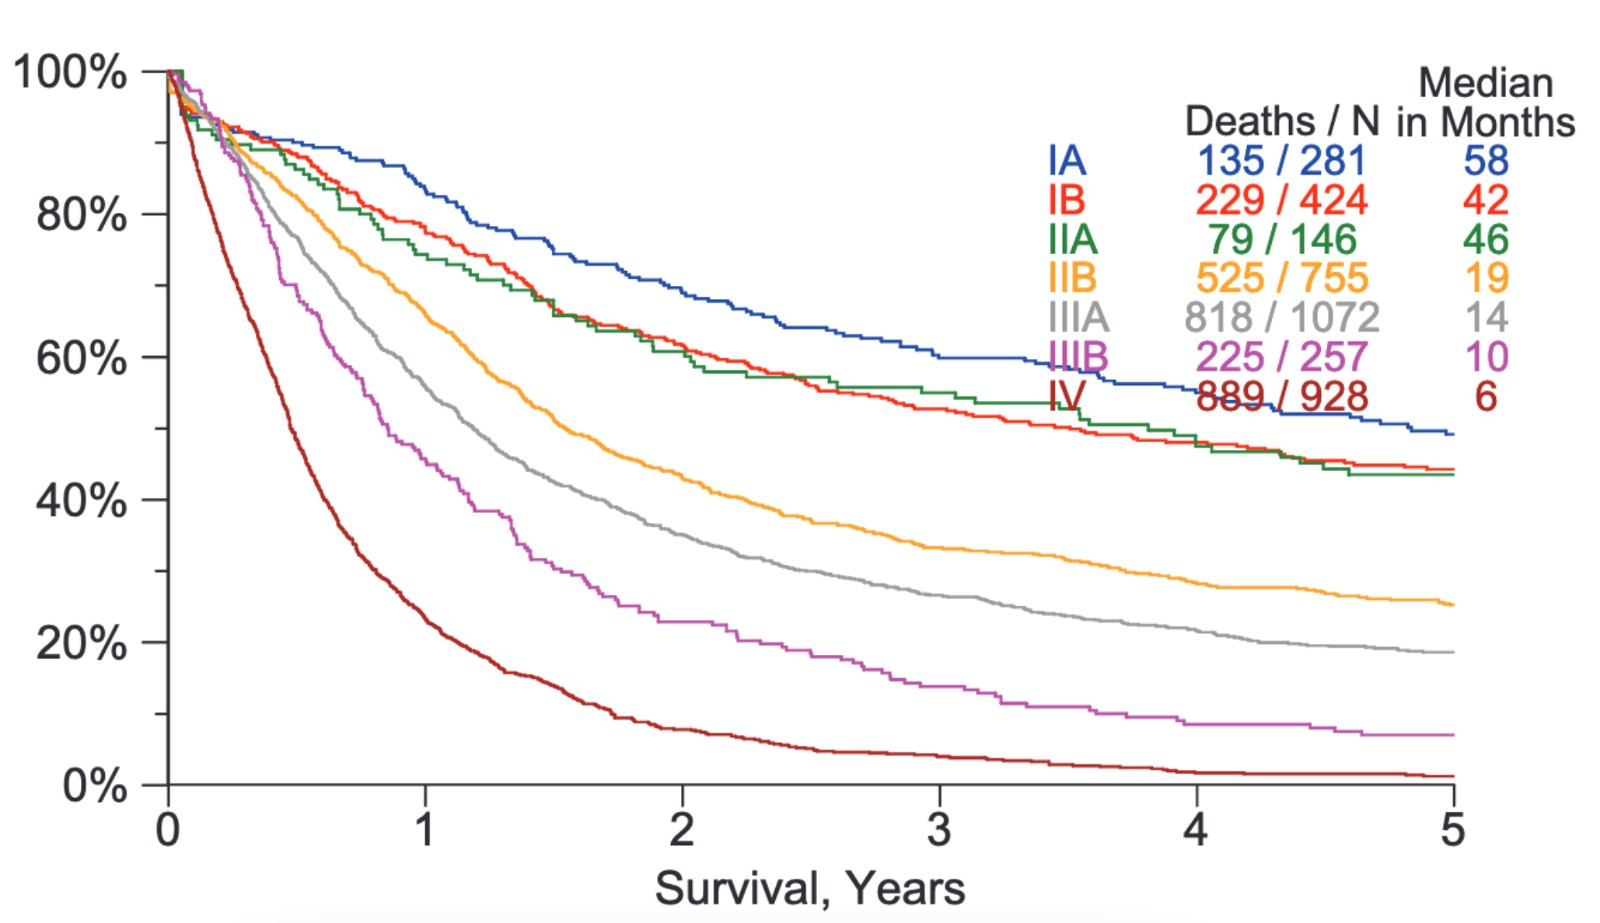
\includegraphics[width = 0.75\textwidth]{groome.jpeg}}
	\caption{5-year-survival probability by lung cancer stage; taken from Figure 6A in \cite{groome2007}}
\end{figure}
\end{frame}


\begin{frame}{Scenario 1: Categorical Representation}
\begin{itemize}
\item Let variable $X^*$ be a major driver of treatment effect heterogeneity.
\item We don't observe $X^*$, but a categorical version thereof, $X$.
\item The important variable \textit{Stage} in cancer data is categorical!\bigskip
\end{itemize}

How to simulate this?
\begin{itemize}
	\item Generate continuous $X^*$ measuring cancer severity;
	\item Group $X^*$ into groups based on its quantiles;
	\item The group membership $X$ (= Stage) is observed.\bigskip
\end{itemize}
Procedure generalizes to non-cancer applications.\\\bigskip
\textcolor{emc-darkblue}{\ding{212}} \alert{Does categorical representation affect model's performance?}
\end{frame}



\begin{frame}{Scenario 2: Undersampling of Subgroups}
\alert{Motivation:} Females and non-Whites are often underrepresented in trials.\medskip
\begin{itemize}
	\item 2010 US Census: 72\% of Americans are White and 13\% African-American.\medskip
	\item Case study: In the largest clinical trial on lung cancer screening:\medskip
	\begin{itemize}\setlength\itemsep{0.5em}
	\item 90\% of participants are White and 4.5\% African-American.
	\item 59\% are male, 41\% female.
	\item Source: \cite{nlst2011}.
	\item Possible heterogeneity along ethnicity \citep{blom2020}.\bigskip
	\end{itemize}
\item[\ding{212}] \alert{Does undersampling affect model's ability to capture heterogeneity?}
\end{itemize}
\end{frame}


\begin{frame}{Scenario 2: Undersampling of Subgroups}
Luckily, this issue has recently started to attract public attention:
	\begin{figure}
		\frame{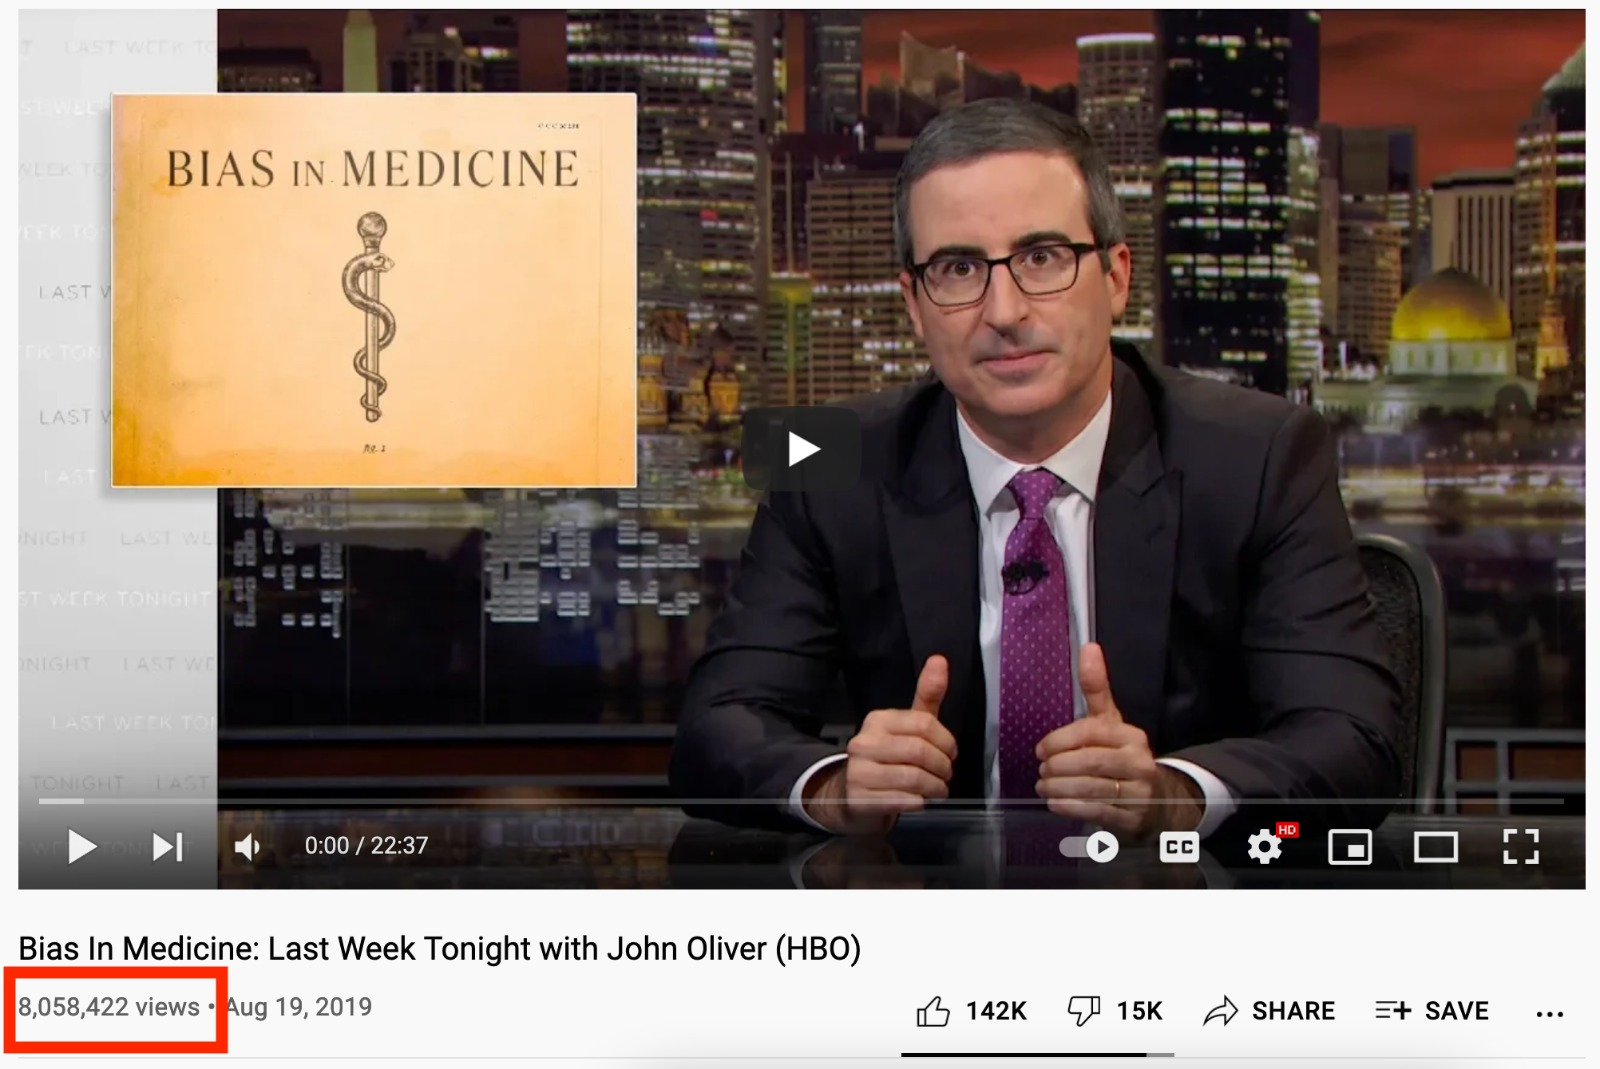
\includegraphics[width = 0.83\textwidth]{oliver.jpeg}}
	\end{figure}
\end{frame}


\begin{frame}{Scenario 3: Nonlinearity}
Recall the potential mortality probabilities:
\[
\pi_i(W) = \P[Y_i(W)=1 | W_i, \X_i] = F_{logistic}\Bigg( \theta(\X_i)W +  \nu (\X_i) + \varepsilon_i \Bigg).
\]
The HTE and nuisance functions ($\theta(\cdot)$ and $\nu(\cdot)$) may be nonlinear.\medskip \\ 
We consider various degrees of nonlinearity:\medskip
\begin{itemize}\setlength\itemsep{1em}
	\item E.g. quadratic, exponential, logarithmic, a mix thereof;
	\item Nonlinear interactions of variables;
	\item Baseline is linearity.\bigskip
\end{itemize}

\textcolor{emc-darkblue}{\ding{212}} \alert{Does degree of nonlinearity affect model's performance?}
\end{frame}


\begin{frame}{Scenario 4: Sparsity}
The HTE function $\theta(\X_i)$ may effectively only depend on a subset of $\X_i$.\\
\textcolor{emc-darkblue}{\ding{212}} Not all variables affect treatment effectiveness. \bigskip\\
Easiest example: Assume linearity in parameters, i.e.
\[
	\theta(\X_i) = \X_i^\top \bm{\beta} = \beta_1X_{i,1} + \dots + \beta_pX_{i,p},
\] 
where $\bm{\beta} \in \mathbb{R}^p$ is fixed and sparse. \\ \bigskip
\textcolor{emc-darkblue}{\ding{212}} Only variables with nonzero coefficient matter for HTE.\\
\textcolor{emc-darkblue}{\ding{212}} \alert{Can the model identify these variables?}
\end{frame}


\begin{frame}{Scenario 5: Anomalous Individuals}
\begin{itemize}\setlength\itemsep{1em}
\item There may be individuals with extreme characteristics.
\item For example: extreme smokers ($\geq100$ cigarettes/day!) or extremely obese individuals.
\item Often, such individuals are at extreme mortality risk, regardless of treatment assignment status.
\item[\ding{212}] \alert{Can a few extreme individuals affect the model's fit?}
\end{itemize}

\end{frame}


\section{Estimation: Considered Methods}


\begin{frame}{Overview: Methods for Estimating HTE}

Methods from medicine:
\begin{itemize}
\item Rate ratios;
\item Predictive modeling: risk \& effect models.\bigskip
\end{itemize}

Methods from stats/metrics:
\begin{itemize}
\item Double Machine Learning \citep{chernozhukov2018double};
\item Generic Machine Learning \citep{chernozhukov2020generic};
\item Causal random forests \citep{athey2019grf}.\bigskip
\end{itemize}

There exist many more; e.g. survival-based models.\\\medskip
You will notice that medical methods are different to causal inference.
\end{frame}


\begin{frame}{Rate Ratios}
\begin{enumerate}
	\item Partition sample in groups $\G_0, \G_1$ you want to compare.
	\item The cumulative times-at-risk of each group are
	\[
		N_0 = \sum_{i\in\G_0} T_i \quad \text{ and } \quad N_1 = \sum_{i\in\G_1} T_i.
	\]
	\item Define fatality counting variables 
	\[
		P_0 = \# \{i \in \G_0 : Y_i = 1\} \quad \text{ and } \quad P_1 = \# \{i \in \G_1 : Y_i = 1\}.
	\] 
	\item Assume
	\[
		P_0\sim Poisson(N_0\lambda_0) \quad \text{ and } \quad P_1\sim Poisson(N_1\lambda_1)
	\]
	for fixed, but unknown $\lambda_0,\lambda_1 > 0$.
\end{enumerate}
\end{frame}


\begin{frame}{Rate Ratios}
\begin{enumerate}\setcounter{enumi}{4}
	\item We are interested in inference on the \textit{rate ratio}
	\[
		\xi = \lambda_0 \big/ \lambda_1.
	\]
	\item Test $H_0: \xi = 1$ against $H_1: \xi \neq 1$ by UMP test (e.g. \citealp{lehmann1986}).
	\item If $H_0$ is rejected, there is evidence for systematic mortality differences between the two groups: means that treatment effect is different between them.
\end{enumerate}
\end{frame}

\begin{frame}{Rate Ratios}
\begin{itemize}\setlength\itemsep{1em}
	\item Rate ratios are also called ``one-variable-at-a-time'' analyses.
	\item Heavily criticized by recent literature \citep{kent2020path}: e.g. low power, multiplicity.
	\item Nevertheless, still common method for HTE identification in medicine.
	\item But: Literature admits that better methods are required (e.g. \citealp{kent2020path}).
\end{itemize}
\end{frame}


\begin{frame}{Predictive Risk Models}
Risk models \citep{kent2020path} are a two stage approach to identify HTE.
\begin{enumerate}
	\item Stage 1: Fit logistic regression model (w/o treatment variable!)
	\[
	\log \Bigg( \frac{\P[Y_i = 1 | \X_i]}{1 - \P[Y_i = 1 | \X_i]} \Bigg)
	=
	\beta_0 + \X_i^\top \bm{\beta}
	\]
	and calculate $\widehat{\eta}_i = \widehat{\beta_0} + \X_i^\top \widehat{\bm{\beta}}$.
	\item Stage 2: Fit the logistic regression model
	\[
	\log \Bigg( \frac{\P[Y_i = 1 | \X_i, W_i, \widehat{\eta}_i]}{1 - \P[Y_i = 1 | \X_i, W_i, \widehat{\eta}_i]} \Bigg)
	=
	\gamma_0 + \gamma_1 W_i + \gamma_2 \widehat{\eta}_i + \gamma_3 \widehat{\eta}_i W_i.
	\]
	\item Calculate predicted risk \[risk_i(W) = \widehat{\P}[Y_i = 1 | \X_i, W, \widehat{\eta}_i].\]
\end{enumerate}
\end{frame}


\begin{frame}{Predictive Risk Models}
\[
	\log \Bigg( \frac{\P[Y_i = 1 | \X_i, W_i, \widehat{\eta}_i]}{1 - \P[Y_i = 1 | \X_i, W_i, \widehat{\eta}_i]} \Bigg)
	=
	\gamma_0 + \gamma_1 W_i + \gamma_2 \widehat{\eta}_i + \gamma_3 \widehat{\eta}_i W_i.\bigskip
	\]
\begin{itemize}\setlength\itemsep{1em}
	\item Idea behind two stages: Separate the explanatory power for $Y_i$ into a part that is due to $X_i$ and a part due to $W_i$.
	\item If treatment is effective, then $H_0: \gamma_1 = 0$ should be rejected.
	\item If there is heterogeneity, then $H_0: \gamma_3 = 0$ should be rejected.
	\item Predicted risk $risk_i(W) = \widehat{\P}[Y_i = 1 | \X_i, W, \widehat{\eta}_i]$ can be used for HTE identification (more on this later).
\end{itemize}
\end{frame}


\begin{frame}{Predictive Effect Models}
Effect models \citep{kent2020path} rely on variable selection to identify heterogeneity.
\begin{enumerate}
	\item Specify set $\mathcal{I} \subseteq \{1,\dots,p\}$ of covariates to interact $W$ with.
	\item Consider the logistic regression model
	\[
	\log \Bigg( \frac{\P[Y_i = 1 | \X_i, W_i]}{1 - \P[Y_i = 1 | \X_i, W_i]} \Bigg)
	=
	\beta_0 + \X_i^\top \bm{\beta} + \gamma_0 W_i + \sum_{j\in\mathcal{I}} \gamma_j W_i X_{i,j}.
	\]
	\item Fit the model using a regularization penalty on coefficient size (e.g. elastic net; \citealp{zou2005}).
	\item Calculate predicted risk \[risk_i(W) = \widehat{\P}[Y_i = 1 | \X_i, W].\]
\end{enumerate}
\end{frame}

\begin{frame}{Predictive Effect Models}
\[
	\log \Bigg( \frac{\P[Y_i = 1 | \X_i, W_i]}{1 - \P[Y_i = 1 | \X_i, W_i]} \Bigg)
	=
	\beta_0 + \X_i^\top \bm{\beta} + \gamma_0 W_i + \sum_{j\in\mathcal{I}} \gamma_j W_i X_{i,j}. \bigskip
\]

\begin{itemize}\setlength\itemsep{1em}
	\item If treatment is effective, then $W_i$ should be selected;
	\item If there is heterogeneity along the variables in $\mathcal{I}$, these variables should be selected. 
	\item We recommend to use a regularization penalty akin to \cite{bien2013} to account for special hierarchical structure of interaction effects.
\end{itemize}
\end{frame}


\begin{frame}{Obtaining HTE estimates}
\alert{Given:} Predicted risk $risk_i(W)$ in risk or effect model.\\\medskip
\alert{Goal:} Estimate HTE $\tau_i = \pi(1) - \pi(0)$ to identify heterogeneity.\bigskip

\begin{itemize}
\item Define the \textit{reversed} treatment assignment
\[
	W_i^{rev} = 
	\begin{cases}
	1 \quad &\text{if } W_i = 0;\\
	0 \quad &\text{if } W_i = 1.
	\end{cases}
\] 
\item Estimate $\tau_i$ via
\[
	\widehat{\tau}_i = risk_i(W_i) - risk_i(W_i^{rev}).
\]
\item Thereupon, one can obtain estimates of $ATE_{\G}, ARTE_{\G}$.
\end{itemize}
\end{frame}

\section{Discussion}

\begin{frame}{Outlook}
In CITRUS, we point out problems. We do not (yet) propose methodological solutions.\\ 
\textcolor{emc-darkblue}{\ding{212}} \alert{Potential for many valuable novel contributions!} For example,

\begin{itemize}\setlength\itemsep{1em}
	\item Derive valid confidence intervals for risk model coefficients (2SLS literature?)
	\item Derive probability of selecting all correct variables in effect model (build on \cite{bien2013}?)
	\item Derive valid confidence intervals for effect model coefficients (build on \cite{dezeure2015} and \cite{vandegeer2016estimation}?)
	\item Valid subgroup-level inference (build on \cite{guo2021}?)
	\item Robustify regression (also in survival models!) (build on \cite{lecue2020}?)
\end{itemize}
\end{frame}

\begin{frame}{Outlook}
\begin{center}
\Huge{We are hiring! (In some way\dots)}
\end{center}

\begin{center}
We might want to start working on some of these extensions in the future (EUR and EMC plan to intensify their collaboration). \bigskip
\end{center}

\begin{center}
\LARGE{\alert{Let us know if you are interested!} \\(It's fine if you are in AMS)}
\end{center}
\end{frame}

\begin{frame}
\centering \Huge{Thank you for your attention! Any questions?}
\end{frame}



\begin{frame}[t,allowframebreaks]
\frametitle{References}
\bibliography{bibliography}
\end{frame}

\end{document} % remove survival time; only makes notation more complicated, as you'd need to incorportate a time dimension in the tretament-induced mortality reduction